\appendix
\part*{Annexes}
\addcontentsline{toc}{part}{Annexes}
\pagestyle{myheadings}
\markboth{Annexes}{Annexes}

\section{Disponibilité des données du mémoire}\label{code}

Illustrations, code et données du mémoire disponibles sur Github à cette adresse : \url{https://github.com/CamillePerault/Agency_in_language__an_evolutionary_perspective}. 

Version \LaTeX disponible sur Github, à cette adresse \url{https://github.com/CamillePerault/redaction_Agency_in_language__an_evolutionary_perspective}.

\section{Annexe psycho-linguistique}\label{Vallacher_grille}

\begin{figure}[!ht]
    \centering
    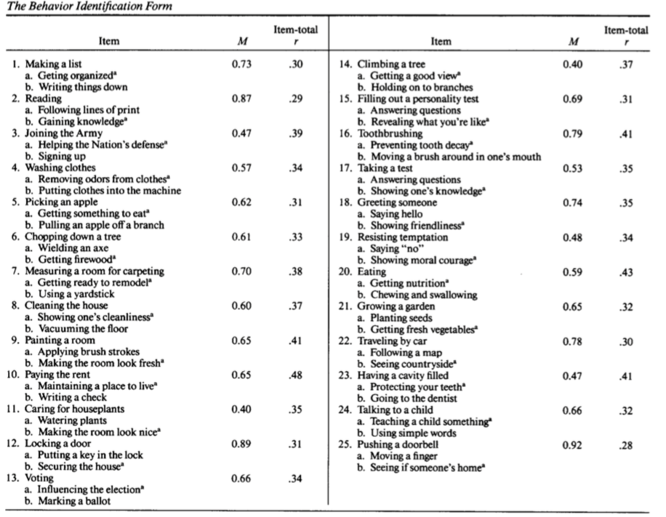
\includegraphics[width=15cm]{img/Vallacher_grille_annexe.png}
    \caption{Le « formulaire d'identification des comportements » utilisé par Vallacher (1989) afin d'estimer le degré d'agentivité de ses participants}
    \label{lm_statut}
\end{figure}

\newpage
\section{Résultats détaillés des modèles de régression}\label{result_models}

\begin{figure}[!ht]
    \centering
    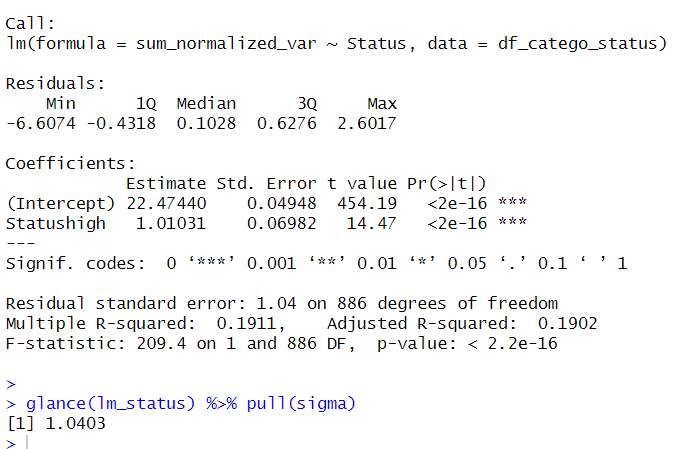
\includegraphics[width=12cm]{img/lm_statut.png}
    \caption{Résultats de la régression linéaire prédisant le score agentif par le statut - modèle 1}
    \label{lm_statut}
\end{figure}

\begin{figure}[!ht]
    \centering
    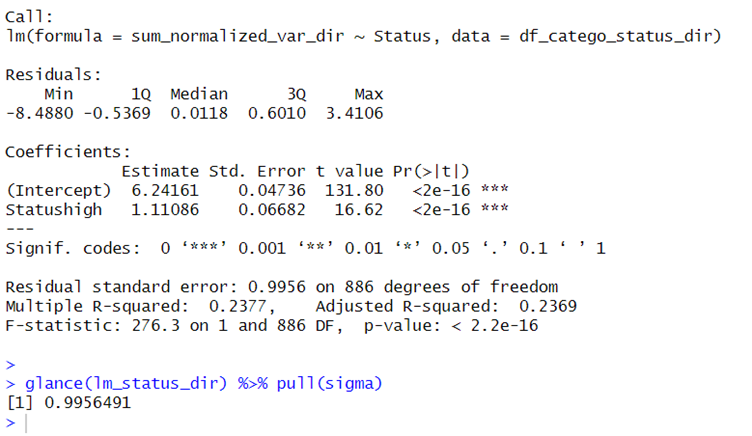
\includegraphics[width=12cm]{img/lm_statut_dir.png}
    \caption{Résultats de la régression linéaire prédisant le score agentif par le statut - modèle 2}
    \label{lm_statut_dir}
\end{figure}

\begin{figure}[!ht]
    \centering
    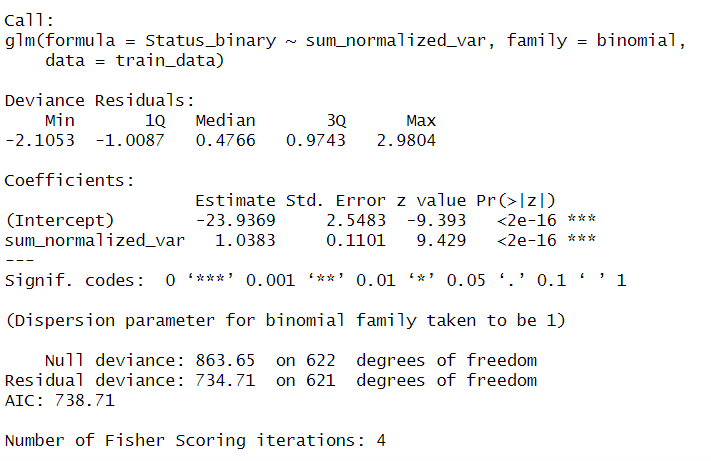
\includegraphics[width=12cm]{img/logit_statut.png}
    \caption{Résultats de la régression logistique prédisant le statut par le score agentif - modèle 1}
    \label{logit_statut}
\end{figure}

\begin{figure}[!ht]
    \centering
    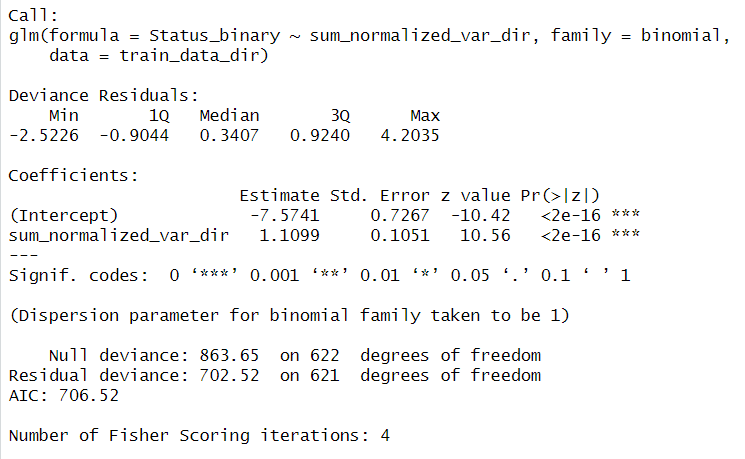
\includegraphics[width=12cm]{img/logit_statut_dir.png}
    \caption{Résultats de la régression logistique prédisant le statut par le score agentif - modèle 2}
    \label{logit_statut_dir}
\end{figure}

\begin{figure}[!ht]
    \centering
    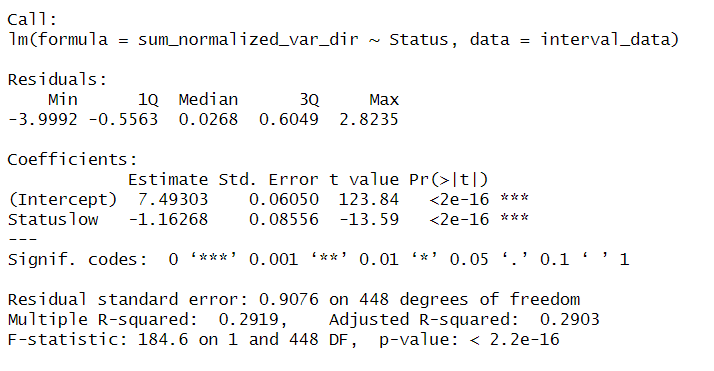
\includegraphics[width=12cm]{img/lmer1.png}
    \caption{Résultats du modèle linéaire hiérarchique intégrant l'effet de l'année de publication à la prédiction du score agentif par le statut - modèle 1}
    \label{lmer1}
\end{figure}

\begin{figure}[!ht]
    \centering
    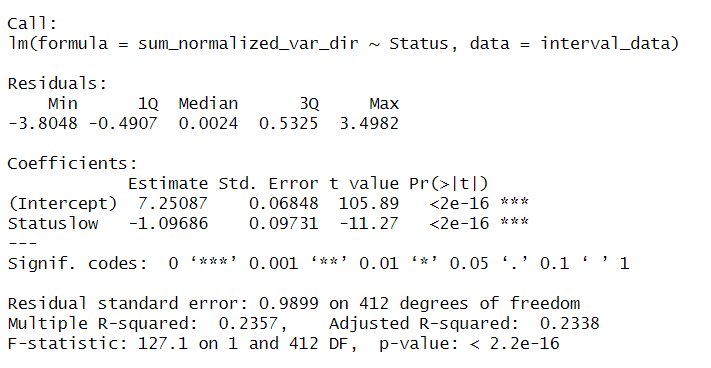
\includegraphics[width=12cm]{img/lmer2.png}
    \caption{Résultats du modèle linéaire hiérarchique intégrant l'effet de l'année de publication à la prédiction du score agentif par le statut - modèle 2}
    \label{lmer2}
\end{figure}